\subsection{Java Plugin}
Prima di tutto è necessario indicare in che linguaggio il nostro progetto viene rilasciato (consideriamo d'ora in poi solo il caso di Java), possiamo farlo in 2 modi:
\begin{enumerate}
    \item aggiungere al file build.gradle:
    \begin{lstlisting}[frame=single]
apply plugin: 'java' \end{lstlisting}
    \item aggiungere al file build.gradle:
    \begin{lstlisting}[frame=single]
plugins {
    id 'java'
}
    \end{lstlisting}
\end{enumerate}
Questo aggiungerà vari tasks necessari ad un progetto in java:
\begin{figure}[H]
    \centering
    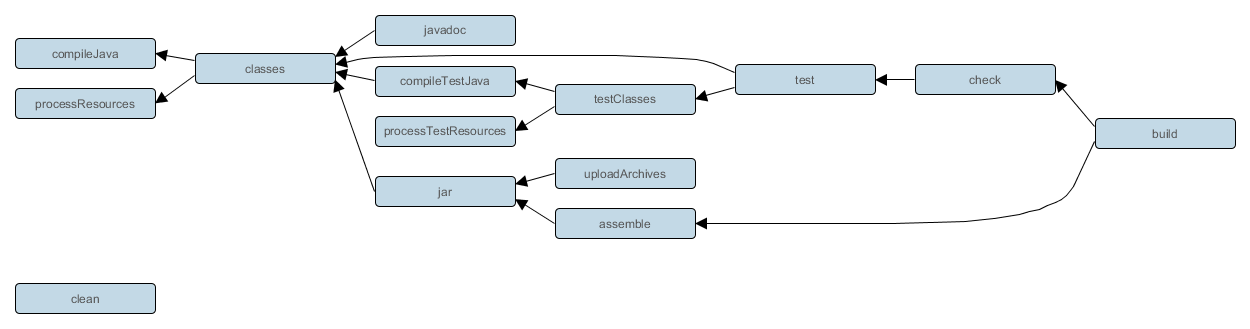
\includegraphics[width=1.0\linewidth]{3DependencyManagement/javaPlug/javaPluginTasks.png}
\end{figure}
A questo punto per poter usufruire di una dipendenza è necessario specificare da dove Gradle deve andare a prenderla, dobbiamo quindi indicare il repository remoto di riferimento. Se per esempio vogliamo che il nostro repository di riferimento sia Maven allora dobbiamo aggiungere al build.gradle:
\begin{lstlisting}[frame=single]
repositories {
    mavenCentral()
} \end{lstlisting}
In questo modo tutte le dipendenze che andremo a indicare successivamente saranno riferimenti alle pubblicazioni su Maven Central. La dichiarazione delle dipendenze deve essere inserita nel tag \texttt{dependencies} nel build.gradle file. Per esempio vogliamo avere junit 4.12 come dipendenza al nostro progetto Gradle allora dobbiamo aggiungere:
\begin{lstlisting}[frame=single]
dependencies {
    testImplementation group: 'junit', name: 'junit', version: '4.12' 
} \end{lstlisting}
Osserviamo che nella dichiarazione ci sono 4 diversi indicatori:
\begin{itemize}
    \item \texttt{testImplementation} indica la configurazione della dipendenza, in questo caso sarà importata durante l'implementazione dei test;
    \item \texttt{group, name, version} corrispondono rispettivamente al groupId (nome del team o della società che ha sviluppato il modulo), artifactId (nome effettivo del modulo) e al version (versione del modulo) definiti su Maven.
\end{itemize}
Esiste un modo molto più diretto per indicare una dipendenza:
\begin{lstlisting}[frame=single]
dependencies {
    testImplementation 'junit:junit:4.12'
} \end{lstlisting}
Ha lo stesso significato precedente ma ha una forma più compatta, forma che adotta anche la documentazione Maven:
\begin{figure}[H]
\centering
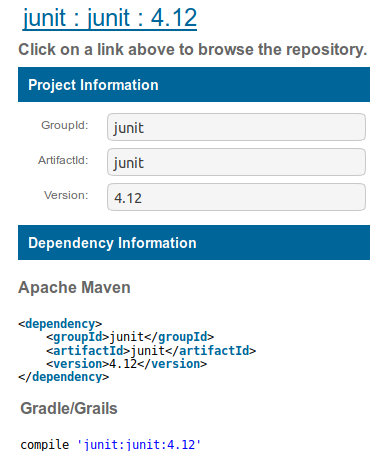
\includegraphics[width=0.4\linewidth]{3DependencyManagement/javaPlug/gradleInMavenRepo.png}
\end{figure}
Spesso in un progetto non è necessario specificare il numero dell'aggiornamento della versione, ma basta la versione più aggiornata, questo è possibile indicarlo a gradle con un \texttt{+} subito dopo la versione voluta:
\begin{lstlisting}[frame=single]
dependencies {
    testImplementation 'junit:junit:4.+'
} \end{lstlisting}
In questo modo quando eseguiremo il task \texttt{dependencies} gradle si assicurerà che la versione in uso di quella dipendenza specifica sia l'ultima rilasciata. Possiamo notare ora la differenza sostanziale della configurazione delle dipendenze tra il pom.xml di Maven e il build.gradle di Gradle. A questo punto per scaricare le dipendenze si deve eseguire il comando \texttt{dependencies} il cui output restituirà una lista di tutte le configurazioni con le relative dipendenze associate (non mostro tutto l'output perchè è molto corposo):
\begin{verbatim}
> Task :dependencies 

------------------------------------------------------------
Root project
------------------------------------------------------------

[...]

compile - Dependencies for source set 'main' (deprecated, use 'implementation ' instead).
No dependencies

[...]

default - Configuration for default artifacts.
No dependencies

[...]

runtime - Runtime dependencies for source set 'main' (deprecated, use 'runtimeOnly ' instead).
No dependencies

[...]

testCompileClasspath - Compile classpath for source set 'test'.
\--- junit:junit:4.+ -> 4.12
     \--- org.hamcrest:hamcrest-core:1.3

testCompileOnly - Compile only dependencies for source set 'test'.
No dependencies

testImplementation - Implementation only dependencies for source set 'test'. (n)
\--- junit:junit:4.+ (n)

testRuntime - Runtime dependencies for source set 'test' (deprecated, use 'testRuntimeOnly ' instead).
No dependencies

testRuntimeClasspath - Runtime classpath of source set 'test'.
\--- junit:junit:4.+ -> 4.12
     \--- org.hamcrest:hamcrest-core:1.3

[...]

BUILD SUCCESSFUL in 0s
1 actionable task: 1 executed \end{verbatim}
Come è possibile notare dall'output esistono molte configurazioni associabili a una dipendenza: compile, default, runtime, testImplementation, e così via, ognuno dei ha uno scopo ben preciso. Possiamo dividere le configurazioni in 3 scopi principali:
\begin{enumerate}
    \item \texttt{implementation}, sono le dipendenze necessarie per compilare il source del progetto che non devono comparire nell'API
    \item \texttt{api}, sono le dipendenze necessarie per compilare il source del progetto che devono comparire nell'API
    \item \texttt{testImplementation}, sono le dipendenze necessarie per compilare ed eseguire i test associati alla source del progetto
\end{enumerate}
I tasks aggiunti da questo plugin assume che il layout del progetto sia di questo tipo:
\begin{center}
\begin{tabular}{|c|c|}
\hline
Directory & Meaning  \\
\hline
\hline
    src/main/java & Sorgente del codice Java\\
    src/main/resources & Risorse \\
    src/test/java & Sorgente del codice di Test \\
    src/test/resources & Risorse usate dai test \\
\hline
\end{tabular}
\end{center}
Tutto questo è automatizzato dal comando:
\begin{verbatim}
    $ gradle init --type java-application\end{verbatim}
Che creerà lo scheletro di un progetto standard Java per sviluppare un applicativo (nel caso si voglia sviluppare una libraria si deve usare il tipo \texttt{java-library}). Il task sicuramente più usato in un progetto è \texttt{test}, questo task è una istanza della classe \texttt{Test} definita da Gradle (consultabile nell'API: \textit{\href{https://docs.gradle.org/current/dsl/org.gradle.api.tasks.testing.Test.html}{docs.gradle.org/current/dsl/org.gradle.api.tasks.testing.Test.html}}) che individua automaticamente tutti gli unit test all'interno della cartella in cui si trova il codice di test, di default nella directory: \texttt{src/test/java}, e li esegue. Può far molto comodo sapere che esiste un opzione \texttt{--continuous} che consente di eseguire un task tutte le volte che viene modificato un file del progetto:
\begin{verbatim}
    $ gradle test --continuous\end{verbatim}
Questo permetterà di controllare ad ogni modifica se la build fallirà o avrà successo. Inolte la build di questo task eseguirà tutti i test dal primo all'ultimo anche se uno di questi fallisce, per progetti di grosse dimensioni quindi questo potrebbe essere uno spreco di risorse. Per indicare alla build di fallire appena un test fallisce ci sono diversi modi:
\begin{enumerate}
    \item Settare la proprietà \texttt{failFast} a true per il task \texttt{test} direttamente nel file di configurazione gradle:
    \begin{lstlisting}[frame=single]
    test {
        failFast = true
    }
    \end{lstlisting}
    \item Indicarlo direttamente da linea di comando, usando l'opzione \texttt{--fail-fast}, nel nostro caso:
\begin{verbatim}
    $ gradle test --fail-fast \end{verbatim}
\end{enumerate}
Questo permetterà di diminuire i tempi di attesa non necessari, facendo fallire al primo test non giusto. Un'altra importante funzionalità di Gradle per quanto riguarda i test è quello di poter specificare dei filtri che indicano con precisione quali test eseguire, per esempio se volessimo eseguire una sola classe di test. Per fare questo ci sono 2 modi:
\begin{enumerate}
    \item Impostare il filtro direttamente nel file di configurazione gradle:
    \begin{lstlisting}[frame=single]
    test {
        filter {
            includeTestsMatching <package>
            includeTestsMatching <methodName>
        }
    }
    \end{lstlisting}
    I filtri supportano anche l'uso delle wildcards "*", per esempio se volessimo eseguire solo gli integration tests e i test del package org.example.app dovremo definire 2 filtri:
    \begin{lstlisting}[frame=single]
    test {
        filter {
            includeTestsMatching "org.example.app.*"
            includeTestsMatching "*IntegTest"
        }
    }
    \end{lstlisting}
    \item Indicare direttamente da linea di comanda per un unica build, usando l'opzione \texttt{--tests}:
    \begin{verbatim}
    $ gradle test --tests <filtro> \end{verbatim}
    Per esempio se volessimo eseguire il metodo di test someFeature della classe SomeTest che si trova nel package org.example.app allora dovremmo eseguire:
    \begin{verbatim}
    $ gradle test --tests org.example.app.SomeTest.someFeature \end{verbatim}
    Oppure volessimo eseguire tutti gli integration tests:
    \begin{verbatim}
    $ gradle test --tests \*IntegTest \end{verbatim}
\end{enumerate}
Ovviamente il secondo caso è quello comunemente usato per eseguire build specifici su una singola classe, evitando di modificare i filtri nel build.gradle. Un altro task importante per il rilascio di un applicativo è \texttt{jar} che crea un file JAR contenente: classi, files e risorse usate. Per essere eseguito questo task necessita la definizione di alcune proprietà:
\begin{itemize}
    \item Titolo del progetto 
    \item Versione del progetto 
    \item Classe in cui si trova il main del progetto (questo viene definito solo nel caso in cui si debba rilasciare un eseguibile) 
\end{itemize}
Queste devono essere inserite nel così detto \textbf{MANIFEST}, andiamo quindi a definire il campo manifest per il task jar:
\begin{lstlisting} [frame=single]
jar {
    manifest {
        attributes("Implementation-Title": "Example",  "Implementation-Version": 1.0, 'Main-Class': 'app')
    }    
}
\end{lstlisting}